\chapter{Web-Based Responsive Spoken Dialogue System}
\label{chap:web-based_responsive_spoken_dialogue_system}

\lettrine{I}{ntroduction} to this chapter\ldots
% complete, web-based \ac{sds} with focus on vocal adaptation.

\pagebreak

\section{Overview and key aspects}
\label{sec:overview_and_key_aspects}

Simulating and triggering accommodation effects occurring in \ac{hhi} like those found in \cref{chap:conv_analysis} in \acp{sds} takes them one step further toward human-like communication.
The system presented in this chapter encapsulates the knowledge acquired from the experiments in \cref{part:experiments}, the behavior designs developed in \cref{part:modeling}, and the module introduced in \cref{chap:convergence_module_for_sdss} which enables the vocal changes.
It contains mechanisms to track the states and changes of segment-level and suprasegmental-level phonetic features during a dialogue.
All the analyses are automated and run in real-time, which not only saves a lot of time and manual work typically needed in convergence studies, but also makes the system more suitable for integration into other applications.
It holds the following key principles:
%
\begin{description}
	\item[Focus on adaptation] --
	the main goal of the system is to offer a tool for investigating vocal accommodation in \ac{hci} for both online experiments and offline analyses.
	Putting vocal accommodation under the spotlight is the core novel contribution of the system, as very few systems offer such capabilities at all, and with control over the accommodative behavior in particular.
	
	\item[Customizability] --
	the system includes several components that can be modified, either for changing the accommodation behavior itself (features, parameters, etc.) or changing the setting (e.g., for different experiments).
	This allows experimenting with different scenarios and configurations and easily compare them in a controlled, reproducible environment.
	
	\item[Online scalability] --
	the system can run in a web browser without any installations or additional files\footnote{some features need to be enabled in the browser, like JavaScript and microphone access.
	However, any modern browser should not have any problem supporting all the necessary requirements.
	To increase performance, all speech analyses and processing are done on the server side.}.
	Since the system itself runs on a single server, it is also possible to operate multiple instances, each with its own configurations and parameters.
	This makes it easy to distribute, e.g., for remotely conducting an experiment where each participant may receive a different configuration.
\end{description}
%
Ultimately, this customizable system could help to deepen the experimental possibilities and automating some aspects of the processes convergence-related experiments typically comprises.
The system's architecture, and \ac{gui}, and functionality are described in \cref{sec:architecture,sec:online_and_offline_paths}.
The experiment presented in \cref{chap:shadowing_experiment_with_natural_and_synthetic_voices} is replicated in \cref{sec:showcase} to demonstrate the system's utilization.

\section{Architecture}
\label{sec:architecture}

As the system aims to offer a customizable playground for experimenting and studying phonetic adaptation in \ac{hci}, a key aspect of its architecture is the separation between client-side, server-side, and external resources (see \cref{fig:web-based_architecture}).
This separation makes it possible to run multiple clients on different machines at the same time with a single server collecting the data from all of them at the same time.
The server, ideally running on a dedicated machine, is operated by an a person responsible of designing and configuring the interactions, e.g., an experimenter.
It collects information and audio recordings from all interactions with the system (which can be deleted afterwards for privacy purposes).
This separation of the server grants the experimenter a lot of freedom and flexibility, since resources like feature configurations and dialogue domain can be modified independently of specific machines interacting with the system.
Additionally, multiple configurations can be prepared in advance (e.g., for different participant groups), regardless of the device the experiment will be performed on and before summoning the participants.
Configurations can even be changed mid-interaction.
These configurations are transparent to the users, and no effort is required from them (aside from start a new interaction in the case of some specific configurations).
This flexibility makes it easier and quicker to create new scenarios of interaction and to experiment with different features and parameters.

In addition to the technical advantages, letting users interact with the system on a separate machine broadens the usage possibilities.
For example, an experiment can be carried out remotely, without the need to invite participants to the recording studio one by one.
Furthermore, as the connection to the server is done via a web browser, participants can connect use the system with their own computers wherever and whenever it suits them, without any additional installation or technical configurations.
All of these makes it possible to collect data from many users rapidly and easily.
%
\begin{figure}[t]
	\centering
	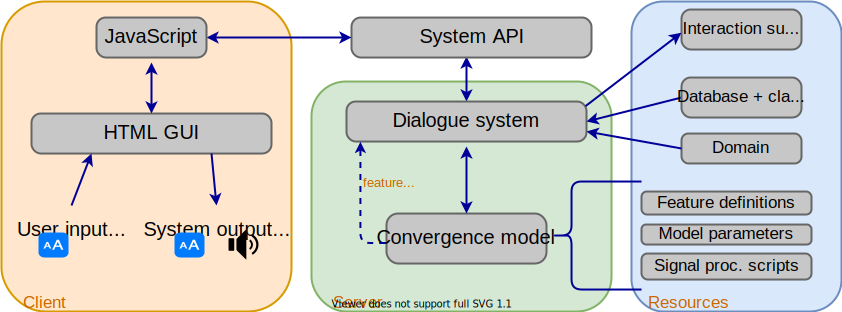
\includegraphics[width=\linewidth]{web-based_architecture_no-ajax}
	\caption[Architecture of a web-based responsive spoken dialogue system]
		{The architecture of the web-based responsive spoken dialogue system.
		The background colors distinguish between client components, server components, and customizable external resources.
		The dashed line indicates that the feature predictions may or may not be passed from the model to the system depending on the feature definition and update parameter.}
	\label{fig:web-based_architecture}
\end{figure}
%
As shown in \cref{fig:web-based_architecture}, the main components of the system are the \ac{sds} itself (including the accommodation module; \cref{subsec:dialogue_system}), the \ac{gui} (\cref{subsec:graphical_user_interface}), and the external resources and configuration (\cref{subsec:models_and_cusomizations}).

\subsection{Dialogue system}
\label{subsec:dialogue_system}

The core of the system is the dialogue system component (see \cref{fig:web-based_architecture}), which controls the flow of the interaction, processes user's inputs, and generates the system's responses.
It uses the extended architecture presented in \cref{subsec:extended_sds}, which consists of typical \ac{sds} components such as \ac{nlu} and a \ac{dm}, but also contains the \ac{asp} module that adds accommodation support \citep{Raveh2017SemDial}.
The implementation of this module in the system is as described in \cref{fig:adaptation_module_architecture}.
While the \ac{nlu} component uses merely the transcription provided by the \ac{asr}, the \ac{asp} module analyzes the speech signal itself.
Concretely, it tracks occurrences of the defined features and passes their measured values to the convergence model, as explained in \cref{subsubsec:tracked_features}, which, in turn, forwards the tracked feature parameters to the \ac{tts} synthesis component.
The \ac{tts} engine then takes the text generated by the \ac{nlg} component, and, if phonetic-level manipulation is supported, synthesizes the utterance using the values specified by the convergence model.
The connection between the dialogue system's modules is managed by the \emph{OpenDial} framework \citep{Lison2016opendial, Lison2015developing}.
The \ac{asr} module uses CMUSphinx \citep{Lamere2003sphinx} with additional customized functionality for obtaining the phonetic information required for the \ac{asp} module, and the \ac{tts} is driven by MaryTTS \citep{LeMaguer2017uprooted, Schroeder2003mary}.
The \ac{nlu} and \ac{nlg} modules are built using an OpenDial's domain file, as described in \cref{subsubsec:dialogue_domain}.

\subsection{\Acl{gui}}
\label{subsec:graphical_user_interface}

The user interacts with the system via an in-browser \ac{gui} (see \cref{fig:gui}).
At the top of the screen is a control bar, which offers the user overview and easy access to some main functions.
On the left side of the bar, the user can view the list of the interaction's turn history and jump to any of them.
It is also possible to see the list of tracked features and their current state.
Both lists can be reset using the Reset button (in red), which starts a new interaction using the current configurations (which may be changed before pressing the button).
On the other side of the bar, there are buttons for viewing on-screen how-to-use information and changing the settings of the system.
The rest of the \ac{gui} is divided into four areas:
A chat area, where the dialogue is shown,
an interaction area where the user provides input to the systems,
a plot area with interactive dynamic visualization of the tracked features,
and a notification area where prompts for the user can be shown.
The functionality of each is described in \crefrange{subsubsec:chat_area}{subsubsec:notification_area}

\subsubsection{Chat area}
\label{subsubsec:chat_area}

The interaction between the user and the system is shown in a chat-like format at the upper left part of the screen.
Each turn's utterance appears inside a chat bubble with different colors representing the two interlocutors, the user and the system.
The bubbles always contain single utterances, even if the other interlocutor has not spoken between them.
A turn can be replayed at any time using the Play button next to the turn number, corresponding to the turn order on the list accessible from the control bar.
Beside utterance bubbles, the system can also display general-purpose messages in this area, which do not progress the dialogue flow and do count as system utterances.
These messages can be used,
%
\begin{landscape}
	\begin{figure}[t]
		\centering
		\vspace*{-2cm}
		\hspace*{-2cm}
		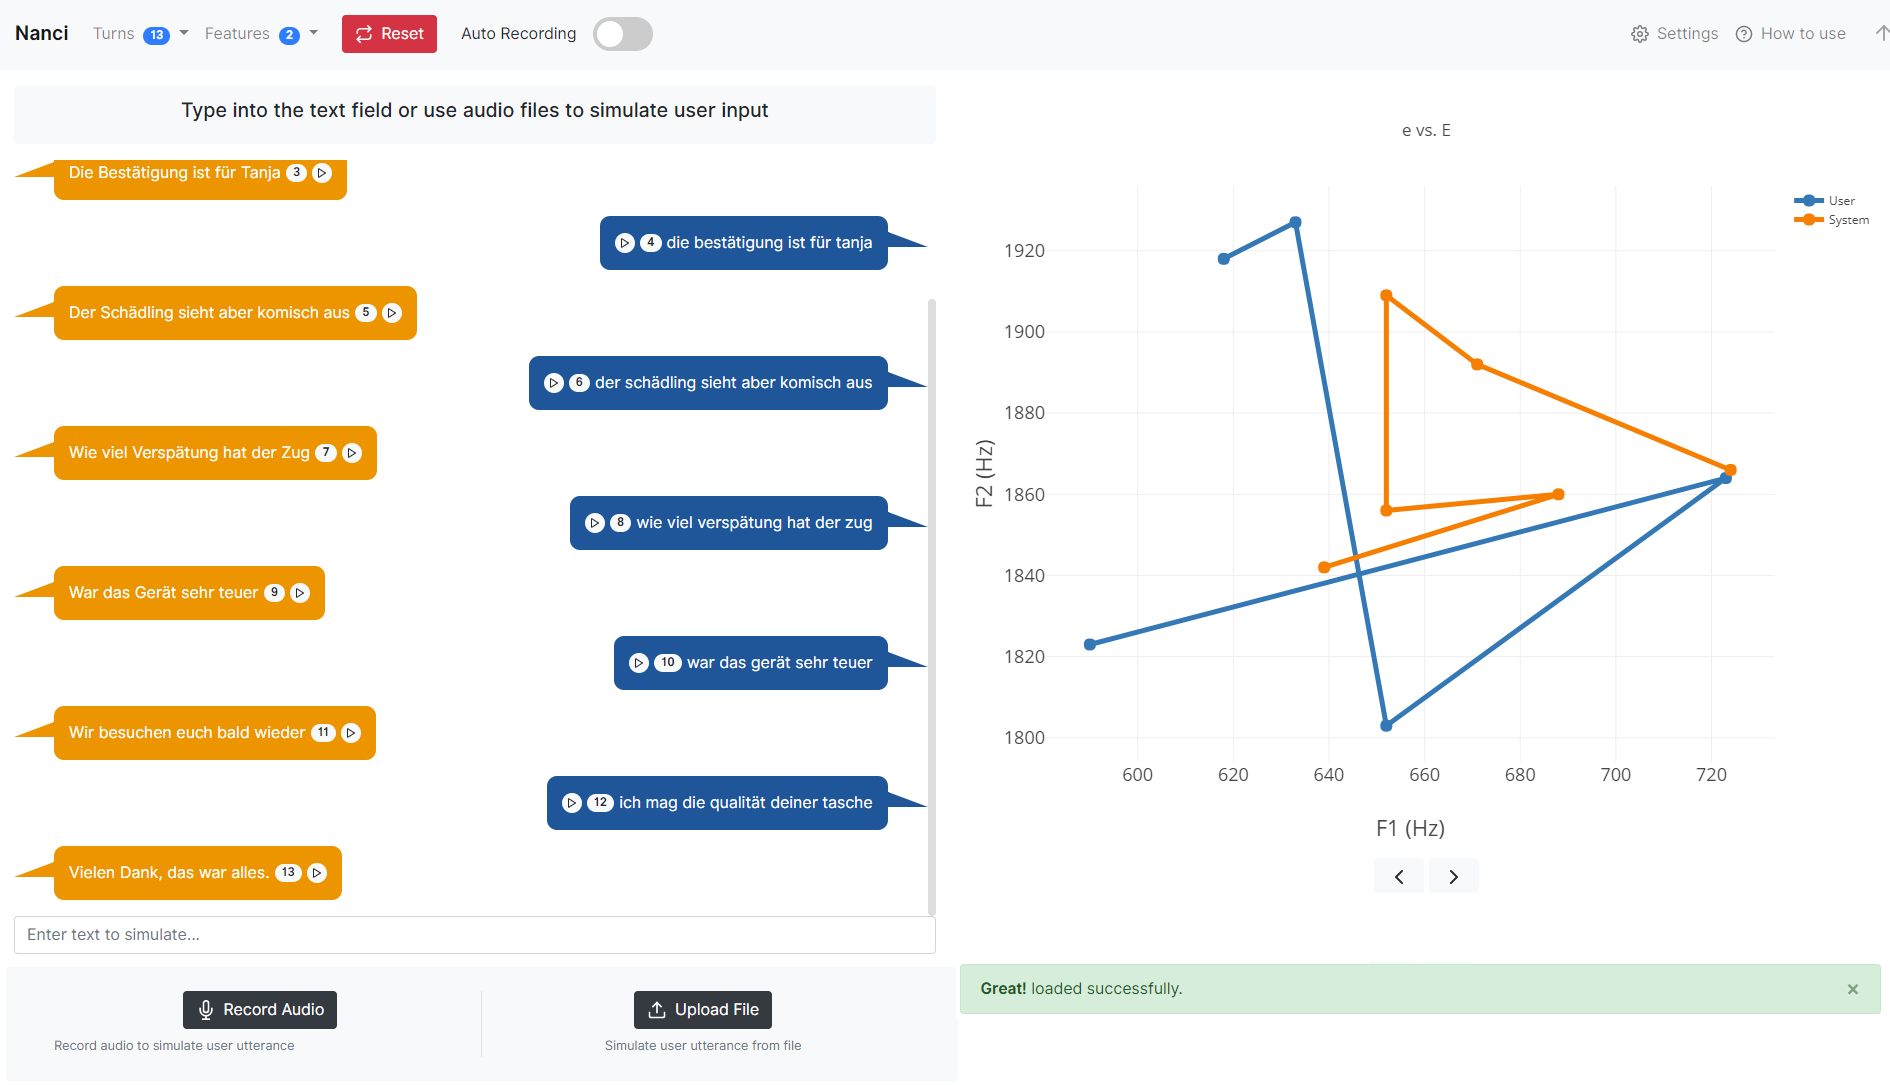
\includegraphics[width=1.6\textwidth]{gui}
		\caption[Web system in-browser \acs{gui}]
			{}
		\label{fig:gui}
	\end{figure}
\end{landscape}
\noindent
for example, to give the user additional information or instructions regarding the interaction.

\subsubsection{Interaction area}
\label{subsubsec:interaction_area}

The user can interact with the system either with either written or spoken input using the controls at the bottom left part of the screen.
Spoken input can be provided either by speaking live into the microphone or via audio files with pre-recorded speech.
These are typically useful for online and offline usage, respectively (\cref{sec:online_and_offline_paths}), but pre-recorded utterances can also be useful for or reproducing previous experiments or comparing different accommodation configurations with the exact same user input.
Text-based interactions progress through the dialogue (if applicable) and trigger any subsequent domain model, but will not affect the tracked features, as no vocal input was provided.
This can be useful for quickly going through specific parts of an experiment (e.g., instructions or setup) or for continuing the dialogue without changing the system's representation of the tracked features.

\subsubsection{Plot area}
\label{subsubsec:plot_area}

\begin{figure}[t]
	\centering
	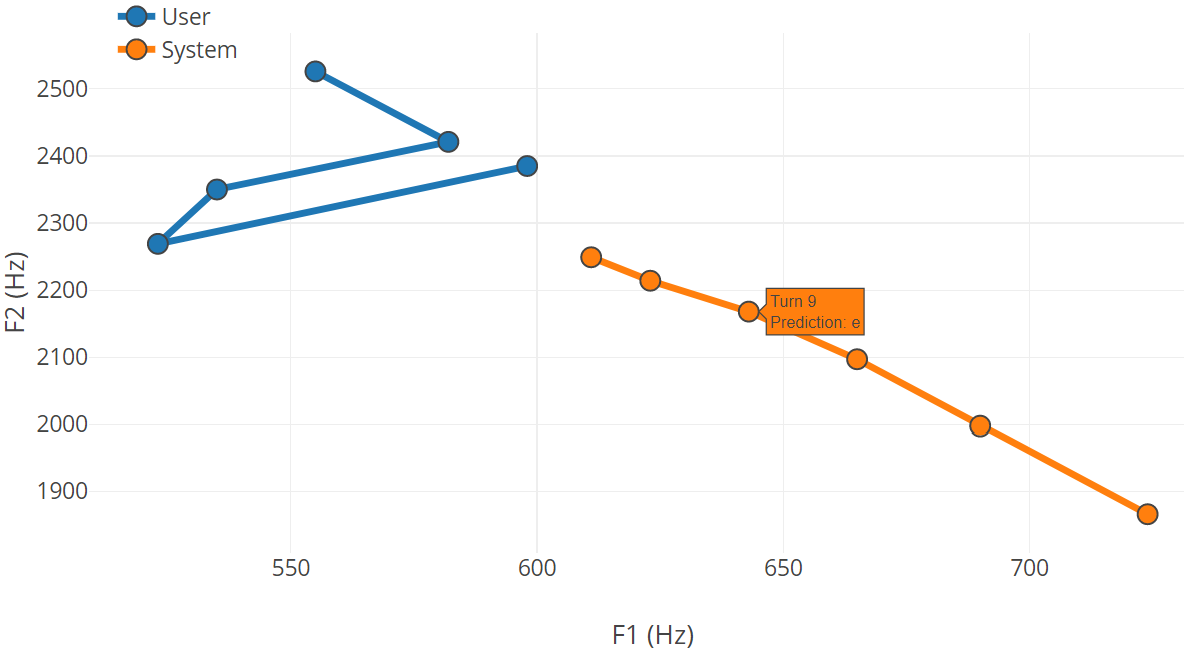
\includegraphics[width=\linewidth]{plot_area}
	\caption[Real-time dynamic visualization of phonetic changes]
		{The plot area showing the states of the feature \textipa{[E:]}~vs.~\textipa{[e:]} during an interaction.
		The system's (orange, bottom right) gradually adapts to the user's (blue, upper left) detected realizations.
		A prediction of the feature's current realization is given for both interlocutors.
		The text box shows the mouse-over annotation of the turn in which the system's realization changes vowel category.}
	\label{fig:plot}
\end{figure}

Visualization of the tracked features' changes over the course of the interaction are displayed in the upper right part of the screen.
Each feature is visualized separately, and new datapoints are dynamically added whenever applicable.
The type of a feature's plot can also change based on its characteristics, e.g., bars for one-dimensional features and lined scatter plots for two-dimensional features.
These plots are generated using the Plotly library\footnote{\url{https://plot.ly}}, which provides some interactive functionalities.
Hovering over a datapoint in the plot reveals additional information, such as the turn in which it was added, or the realized variant of the feature produced in that turn as predicted by its classifier.
\Cref{fig:plot} shows an example of such plot with several accumulated datapoints.

\subsubsection{Notification area}
\label{subsubsec:notification_area}

Whenever a message outside the content of the interaction needs to reach the user, it can be shown at the bottom right part of the screen.
Such messages may include indications of the system's activity, e.g., successful initialization of the interaction, warning and errors while uploading files, or any other prompt the experimenter might want the user to see, like additional instructions to consider during the experiment.
However, the latter is better achieved using the non-speaker turns in the chat area.
The notifications can be colored blue, green, orange, and red to differentiate different types of messages.

%\subsubsection{Settings and help}
%\label{subsubsec:settings_and_help}
%
%An additional modal window can be called, in which various settings can be changed, and some usage information is provided.
%Configurable settings include the convergence model parameters, domain file, \ac{gui} tweaks, and more.
%These settings can be modified at any point during the interaction, so that it is possible to experiment with different configurations in real-time.
%For persistent changes, it is also possible to edit the configuration file itself, which is loaded when the system starts.
%The usage tab explains the various functionalities of the system and how each area of the \ac{gui} works.
%It also lists special commands that can be executed from text field (used for simulating the user's input, as mentioned in \cref{subsubsec:interaction_area}).
%These commands include printing a short or detailed summary of the phonetic changes throughout the interaction, extracting the data from the features' plots (e.g., for further analysis), and more.
%\todo{screenshot with the settings tab}

\subsection{Models and customizations}
\label{subsec:models_and_cusomizations}

The system aims to offer a platform for \acp{sds} with convergence support that can be modified and customized according to the user's needs.
All of the aforementioned system components can be customized to some extent.
This also includes the phonetic convergence model, the features tracked by the system, and the dialogue domain.

\subsubsection{Tracked features}
\label{subsubsec:tracked_features}

The accommodation process is initiated by the phonetic features defined in the configuration file.
There are phonetic features that are prone to variation, and are triggered whenever the \ac{asr} component detects a segment containing a phoneme associated with one or more of these features.
The feature definitions may capture general tendencies or specific phonological rules, like schwa elision in German (see \cref{eq:elision_rule}).
As explained in \cref{subsec:computational_model}, each feature is detected and filtered based on its definition.
This definition can be easily changed to experiment with different accommodation effects.

\subsubsection{Dialogue domain}
\label{subsubsec:dialogue_domain}

The dialogue's flow is specified using OpenDial's XML-based format\footnote{\url{http://www.opendial-toolkit.net/user-manual/dialogue-domains}}.
This format offers a structure for building models, rules, and conditions, which define the \ac{dm} logic.
The rules connect between intents provided by the \ac{nlu} module to textual output generated by the \ac{nlg} module.
Additional parameters are introduced for triggering processing for other modules of the \ac{sds}, like the \ac{asp} module in the system discussed here.
More details about building a domain file can be found in \citet{Lison2016opendial}.
The format of the domain file makes it easy to define new scenarios for the system, like different experiment scenarios.
Rules are written mostly using regular expressions, which makes it possible for non-technical users to design most of the system's logic.
Since the \ac{dm} keeps track of parameters from all modules, the system's output can even be influenced by the state of the accommodation state in the \ac{asp} module (if such information is provided).

\subsubsection{Speech processing}
\label{subsubsec:speech_processing}

Multiple components of the system deal with different aspects of speech processing.
As each module in the system can be replaced independently, different engines and models can be used.
For example, the \ac{asr} engine can be replaced for improving performance or adding support for more languages (that is, all time the same functionality is offered by that engine and the phonemeset used by the system is updated accordingly).
The \ac{tts} component can be replaced as well, e.g., for changing the voice of the system.
Importantly, also the tool used for the phonetic analysis can be changed to improve accuracy or performance.
The models and tools described here are those that were used specifically for the showcase presented in \cref{sec:showcase}.
The \ac{asr} component uses CMUSphinx\footnote{Sphinx4 version 5prealpha, \url{https://cmusphinx.github.io/}} \citep{Lamere2003sphinx}, with an extension to the phoneme emission functionality to provide the \ac{asp} module the input it needs (see \cref{subsec:computational_model}).
The acoustic model and pronunciation dictionary were taken from online CMUSphinx models\footnote{\url{https://sourceforge.net/projects/cmusphinx/files/Acoustic\%20and\%20Language\%20Models/German/}}.
A customized \ac{asr} language model was created with SRILM \citep{Stolcke2002SRILM}).
All the segmental and suprasegmental analyses required for the measuring accommodation were done using Praat \citep{Boersma2018praat}.
MaryTTS \citep{LeMaguer2017uprooted} was used as the \ac{tts} engine of the system, with \texttt{bits1-hsmm} and \texttt{bits3-hsmm} for its female and male voices, respectively.

\section{Online and Offline paths}
\label{sec:online_and_offline_paths}

\begin{figure}[t]
	\centering
	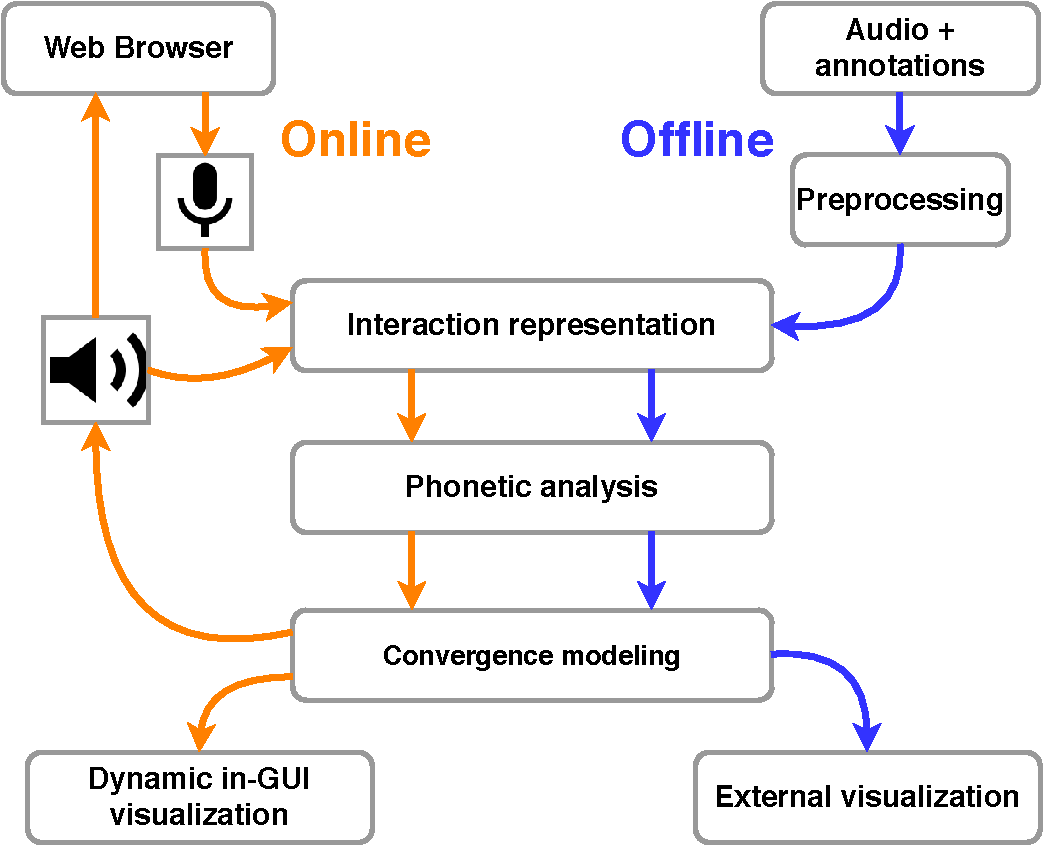
\includegraphics[width=0.85\linewidth]{online_offline_small}
	\caption[Online (orange) and offline (blue) paths of the responsive \acl{sds}]
		{Online and offline paths of the system.}
	\label{fig:online_offline_paths}
\end{figure}

The system can operate in two modes, as shown in \cref{fig:online_offline_paths}:
Online -- turn-based real-time interaction via the \ac{gui} (\cref{subsec:graphical_user_interface}); and offline -- on-demand analysis of already existing interaction data, either from a recorded online sessions or any other dataset.
The accommodation-related parts of the system (roughly corresponding to the \emph{server} and \emph{resources} blocks in \cref{fig:web-based_architecture}) are common to the two paths, which makes it easy to switch between the two.
The differences are in how the data is fed to the system and how the output is processed and visualized.
The main difference is that in the online path the process recurrent and both the user's input and the system's current state are used in the processing of the next turn.
Depending on the scenario defined in the domain file, there could always be another turn, either of the user or the system, to continue the interaction.
In the offline path the data scope is, naturally, pre-defined and finite.
Technically, the dataset is represented and processed the same way as an online interaction, but there is no need to output the system's state to a user.
The common representation also makes it easy to compare pre-recorded interactions with live ones.
The output of the accommodation model after each turn is handled differently in both paths as well.
In online interactions, the output is sent on a turn-by-turn basis to both the web-based \ac{gui} for the different visualizations (as in \cref{fig:plot}) and back to the user for auditory response.
The offline path doesn't need to interact with a user, so the entire analysis is saved together, along with some additional analysis.
This output can then be used for further statistical analysis and be visualized separately using other tools (as in \cref{fig:hds_dds_time_comparisons}).
For using the online mode, the system needs to run as a server and be accessed via a web browser.
The offline mode can be used either directly from the command line or programmatically from another application.
As explained in \cref{subsubsec:interaction_area}, pre-recorded files can also be used from the \ac{gui}.
Using this option for all user inputs would effectively be the same as using the offline path, but would require much more time due to the human manual operation.

\section{Showcase: simulating a shadowing experiment}
\label{sec:showcase}

As a showcase of the system capabilities, it was utilized to replicate the shadowing experiment described in \cref{chap:shadowing_experiment_with_natural_and_synthetic_voices}.
The experiment is designed to trigger and analyze phonetic convergence by confronting the participants with stimuli, in which certain phonetic features are realized in a way different from their own.
This was done using the offline path of the system, to can simulate a real experiment and automate certain parts of it that would otherwise be performed manually.
The replication used the original stimuli and utterances of one of the participants.
However, analyses originally done post facto (and to different extents manually), like detecting the realized variant, measuring the features' values, etc., can be now done automatically.
This demonstrates an automated, reproducible execution, and also offers additional insights via classification of feature realizations and dynamic visualizations in the web \ac{gui} (\cref{subsec:graphical_user_interface}).
Finally, using the system, the experiments becomes dialogue-based rather than a mere experimental setting, which enhances its \ac{hci} nature.

\subsection{Setup adjustments}
\label{subsec:setup_adjustments}

For the experiment simulation, two of the three features investigated in the original experiment (\cref{chap:shadowing_experiment_with_natural_and_synthetic_voices}) were used.
In addition to the \textipa{@}-length feature shown in \cref{subsec:computational_model} the definition of the feature \textipa{[E:]}~vs.~\textipa{[e:]} below was included.
Both features are described in detail in \cref{subsec:target_features_HCIConv} and \cref{tab:target_features} shows example stimuli containing them.
As in the original experiment, the word containing the target features were embedded into 15 short carrier sentences and 25 filler sentences, in which none of the features occur (see \cref{app:shadow_experiment_stimul} for the list of all stimuli).
Although the features' underlying values are gradual, they are perceived as two-way categorical variations.
To map these underlying values to a specific variant, the system associates a classifier with each feature, as explained in \cref{subsec:classifiers_training}.
%
%\begin{description}[labelindent=1.5cm, labelwidth=\widthof{\quad \bfseries calculation}]
%	\item[name]	ee\_E
%	\item[phoneme] EHH
%	\item[context] .* EHH .*
%	\item[initial] 451, 2116, 2763
%	\item[minimum] 300, 1500, 2500
%	\item[maximum] 750, 2900, 4800
%	\item[measure] formants
%	\item[calculation] decaying average
%	\item[sensitivity] 0.3
%\end{description}
%
\begin{Verbatim}[tabsize=4, commandchars=\\\{\}]
	- \textbf{`e\_E\_vowel'}:
			\textbf{phoneme}: EHH
			\textbf{context}: '.* EHH .*'
			\textbf{initial}: 450 2100
			\textbf{minimum}: 300 1500
			\textbf{maximum}: 750 2900
			\textbf{measure}: formants
			\textbf{calculation}: decaying average
			\textbf{sensitivity}: 0.3
\end{Verbatim}
%
%The value of the key \emph{measure} is \enquote{formants}, which means that this feature is evaluated by the segment's formant values (as specified in the corresponding signal processing script).
%The values of the \emph{minimum} and \emph{maximum} keys stand for the acceptable value range for this feature.
%This avoids distorted values due to \ac{asr} error and lets the user put their phonetic expertise to use.
\noindent
The values of the keys \texttt{minimum}, \texttt{maximum}, and \texttt{initial} stand for the first two formant frequencies.
The \texttt{calculation} method for this feature is \emph{decaying average}, which is similar to the regular average but with each value contributing exponentially less to the final value, so that the last (newest) exemplar contributes the most.
Adding such property to the measure gives more weight to new exemplars that were received chronologically closer to the current turn and thus makes the change more strongly influenced by the productions closer to the accommodation change.
Using this measure comes to support the analogy of the exemplar pool to short-term memory, which remembers recent event better than older ones.
Decaying average is defined here as
%
\begin{equation} 
	\label{eq:decaying_average} 
	\mu_n = \frac{1}{n}\sum_{i = 2}^{n}(\eta v_i + (1 - \eta )\mu_{i-1}), 
\end{equation} 
\eqname{Decaying average}
%
\noindent
where $n$ is the number of exemplars in memory, $\eta$ is the decay rate (here, 0.5), $\mu_{i-1}$ is the accumulated decaying average from the previous exemplar, and $v_i$ is the value of the $i$-th exemplar. 

Even though more aspects of it could be automated, the experimental procedure stayed as faithful as possible to the procedure of the original experiment.
The domain file created for the showcase was designed to substitute the role of the experimenter in the shadowing phase (cf.\ \cref{fig:HCIConvFlow}), i.e., presenting -- and speaking -- the next stimulus to the participant.
The stimulus order from the original experiment's baseline phase was preserved and semi-randomized (using the same logic) in the shadowing phase.
It was also configured to perform the transitions between the phases.
Although it should be assumed that the user indeed repeats presented utterance, the system nonetheless verifies that the user's utterance matches the current stimulus using the customized language model described in \cref{subsubsec:speech_processing}

% A shortened example of the shadowing phase's flow is shown in \cref{app:dialogue_example}.

%\begin{description}[labelindent=1.3cm, labelwidth=\widthof{\quad \textipa{[I\c{c}]}~vs.~\textipa{[Ik]}}]
%	\item [\textipa{[E:]}~vs.~\textipa{[e:]}] in word-medial $\langle$ä$\rangle$
%	\item [\textipa{[I\c{c}]}~vs.~\textipa{[Ik]}] in word-final $\langle$-ig$\rangle$
%	\item [\textipa{[\s{n}]}~vs.~\textipa{[@n]}] in word-final $\langle$-en$\rangle$
%\end{description}
%\noindent
%
\begin{table}[t]
	\centering
	\begin{tabularx}{\linewidth}{@{}*{5}{l}}
		\toprule
		
		War          	& das          			& Ger\textbf{\underline{ä}}t	& sehr          	& teuer? \\
		\emph{Was} 		& \emph{the} 			& \emph{device}           		& \emph{very} 		& \emph{expensive?} \\[0.3cm]
		
%		Ich          	& bin         			& sücht\textbf{\underline{ig}}	& nach				& Schokolade. \\
%		\emph{I}   		& \emph{am} 			& \emph{addicted}				& \emph{to} 		& \emph{chocolate.} \\[0.1cm]
		
		Wir         	& besuch\textbf{\underline{en}} 						& euch				& bald          & wieder. \\
		\emph{We} 		& \emph{will visit}		& \emph{you} 					& \emph{soon} 		& \emph{again.} \\
		\bottomrule
	\end{tabularx}
	\caption[Example sentence for selected phonetic features]{Examples of stimuli containing the target features. Each stimulus contains only one feature.}
	\label{tab:target_features}
\end{table}

\subsection{Classifiers training}
\label{subsec:classifiers_training}

The automation the system offers can also be used to provide additional information regarding the realizations of the tracked features, i.e., which category each instance of the feature belongs to.
This automates the annotation otherwise done manually by the experimenter during or after the experiment.
In the shadowing experiment in question, this includes both the determination of the participants' preference in the baseline phase and the annotation of the participants' realizations in the shadowing phase.
To that end, a classifier can be associated with each feature to provide real-time classification for both the user's and the system's realizations of that features.
With this information available, more meaningful insights can be gained into the variation dynamics over the course of the interaction.
In other applications, like \acp{capt}, this information be taken into account when deciding on the system's next turn.
The classifiers for the simulated experiment were trained on a two datasets corresponding to the target features' ranges.
The \textipa{@}-length classifier trained to separate segments shorter and long than \SI{30}{\milli\second}, and the \textipa{e:/E:} classifier was trained on F1 and F2 values of these vowels produced by a set of female speakers.
While training prior to the interactions is sufficient, online fine-tuning is also possible to update a feature's classifier whenever requested by the user, e.g., every time the accommodation model is updated.

Training was performed with a \ac{smo} \citep{Platt1999fast, Platt1998sequential} implementation of the \ac{svm} classifier \citep{Vapnik1998support}.
For multi-dimensional features, multivariate \ac{svm} classification \citep[e.g.,][]{Joachims2005support} was used.
Each turn's predictions dynamically added as interactive annotations to the visualization of the relevant features, as illustrated in \cref{fig:plot}.

\subsection{Validation}
\label{subsec:validation}

\begin{table}[t]
	\centering
	\begin{tabularx}{\linewidth}{X*{4}{S[table-format=2.1]}}
		\toprule
		sensitivity (\numrange{0}{1}) &  0.2 &  0.3 &  0.4 &  0.5 \\
		adoption (\si{\percent})      & 79   & 86   & 75   & 69   \\
		\bottomrule
	\end{tabularx}
	\caption{The system's convergence degree with different degrees of sensitivity.}
	\label{tab:validation_baseline}
\end{table}

%%%%%%%%%%%%%
% text from above. insert somewhere
The validation stays faithful to the original experiment in every possible aspect.
Therefore, the training data used for each classifier contains only the productions of the corresponding target feature from a single stimulus set, since these are the productions to which the participants were exposed during the experiment.
This provides relatively few -- but at the same time very precise -- datapoints for each classifier,
which were obtained using the same signal processing technique as the data collected in the experiment.
%%%%%%%%%%%%%

%The validation for the feature \textipa{[E:]}~vs.~\textipa{[e:]} is shown here as a representative example for the phonetic adaptation capability of the system.
For the baseline phase, the validation examined the degree to which the underlying convergence model accumulated enough data to adopt the user's variant of the feature.
Stronger and quicker adoption indicates a more stable and precise preferred variant of the participant.
The preferred variants of the participant and the system were determined based on the majority vote at the end of this phase, as in the original experiment.
For example, if the user realized one variant twice and another three times, the latter was considered the preferred one.
\Cref{tab:validation_baseline} shows the degree of the model's adoption of the user's preferred variant (translated into percentages of the mean preferred variant) using different values of the \emph{convergence rate} parameter (see \cref{sec:parameters}).
Interestingly, higher values do not necessarily result in higher percentages, due to systematic over-accommodation.
The value 0.3 provided the highest results.% and was therefore used through the rest of the simulation.
%
\begin{figure}[t]
	\centering
	\subfigure[The effect of different convergence rates on the gradual change of
			   the system's representation of a two-dimensional feature \textipa{[e:]} vs.\ \textipa{[E:]} using decaying average ($\mu = 0.3$).
			   The points represent the calculation steps of the rates 0.1 (red circles), 0.5 (yellow tiranlges), and 0.9 (green rectangles).
			   Each point is the new value calculated after accummulating a single exemplar.
			   The first points at the top right are the common initial value.
			   The the ellipses represent confidence levels of \SI{90}{\percent}, \SI{50}{\percent}, and \SI{10}{\percent}, respectively.]
		{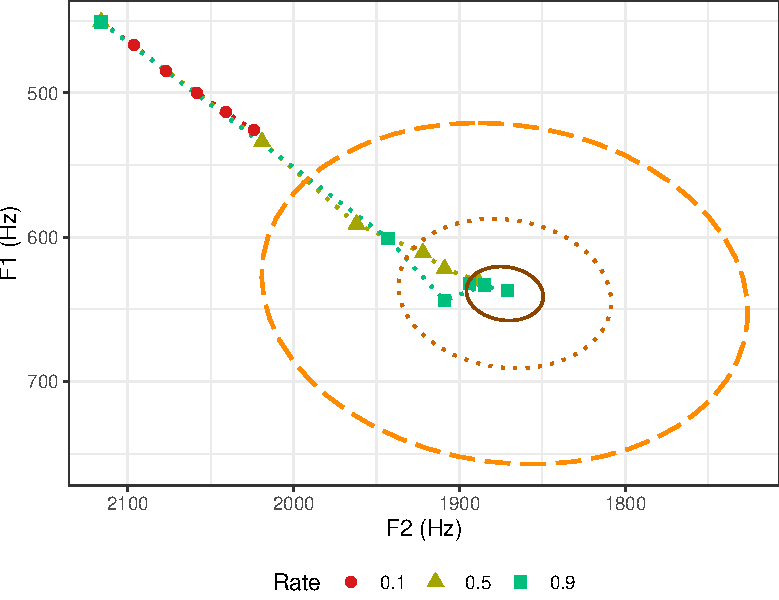
\includegraphics[width=0.47\textwidth]{ee_E_decaying_0.3}
	\label{fig:e_E_bullseye}}
	\hfill
%	\vspace{-1cm}\hfill\hspace{-1cm}{\hbox{\LARGE $\Longrightarrow$}}\hfill
	\subfigure[The effect of different convergence rates with the calculation method set to simple average.
			   The bars' height represent the value of the one-dimensional feature \textipa{@}-length
			   and the numbers on the x-axis are the updates of the feature's representation on each turn.
			   The \emph{exemplar} bar shows the feature’s last exemplar, and the \emph{average} bar
			   is the value of the feature after adding the last exemplar to the pool.
			   Note that the first turn appears empty since the initial value of the feature is 0.]
		{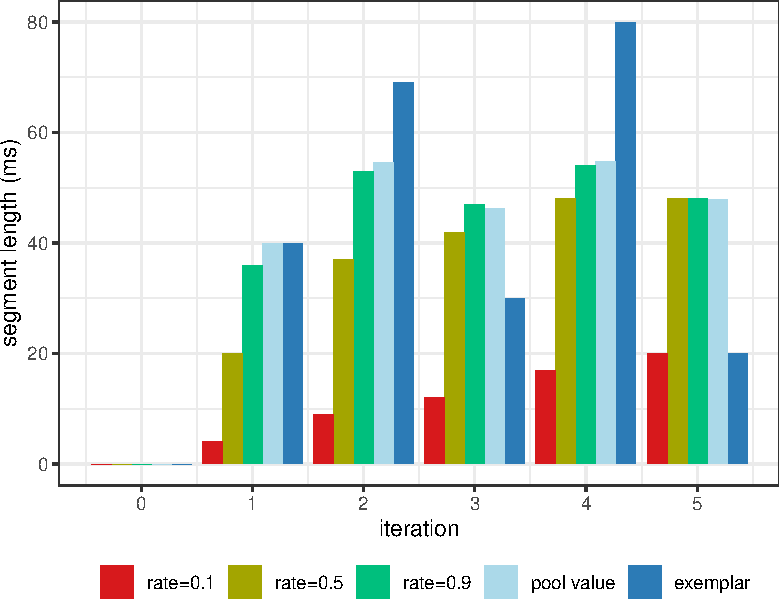
\includegraphics[width=0.47\textwidth]{schwa_comp_010509}
	\label{fig:schwa_length_bars}}
	\caption[Influence of difference convergence rates on the system's accommodation]
		{Illustration of the effect of different convergence rates on the updates of the system's  realization of a two-dimensional feature (left) and a one-dimensional feature (right).}
	\label{fig:validation_sensitivity}
\end{figure}
%
After obtaining the preference of each participant, the degree of convergence was examined per utterance in the shadowing phase.
The participants were grouped based on their convergence behavior in the original experiment:
One group of participants showed low to no tendency to converge (converged in \SI{\le 10}{\percent} of their utterances),
the second had varying degrees of convergence (\SIrange{10}{90}{\percent}),
and a third group of participants who were very sensitive to the stimuli (\SI{\ge 90}{\percent}).
This grouping enables analyses based on collective vocal behaviors instead of individual differences.
The groups are labeled \emph{Low} (\SI{23}{\percent} of participants), \emph{Mid} (\SI{50}{\percent}), and \emph{High} (\SI{27}{\percent}), respectively.
The classifier was determined on the fly, so that the prediction for each utterance was decided based on the stimulus type to which the participant was listening (for instance, a classifier trained on synthetic stimuli was used for participants listening to such stimuli).
For validation purposes, the shadowing phase was treated as an annotation task of the realized variation in the participants' utterances.
The three \enquote{annotators} are the stimuli themselves (\emph{Stim}), the online classification of system's representation of the feature (\emph{Sys}), and additional labels from the training dataset used as references (\emph{Ref}).

The Cohen's kappa ($\kappa$) values\footnote{calculated by the \texttt{kappa2} command of the \texttt{irr} R package v0.84, \url{https://cran.r-project.org/package=irr}} for \emph{Low} are expected to be lower, as a lower degree of convergence was found among these participants.
%As \cref{tab:showcase_results} shows, convergence was found in \SI{48}{\percent} of the utterances for \emph{Sys-Stim} and \emph{Ref-Stim} but only in \SI{66}{\percent} for \emph{Ref-Sys}, which means that convergence was found in different instances.
%\todo{not clear what the sentence above wants to say}
\cref{tab:showcase_results} shows that \emph{Ref-Sys} has $\kappa = 0.2$ (fair agreement) for the \emph{Mid} group, but lower for the other two groups.
This indicates that the reference values, which supposedly represent some universal average of the feature, indeed match the production of the participants that didn't deviate too greatly from their base production values, which reinforces the fact that the stimuli's influence on them was limited to either direction.
The $\kappa$ values for \emph{Sys-Stim} describe how the system's representations matched the stimuli presented to the participants.
Since the system accommodates to the participants' performance, these values exhibit how similarly to the participants of each group the system behaved.
The \emph{High} group achieved $\kappa = 0.81$ (strong agreement), showing that the system became very similar to the users sensitive to changes.
Contrarily, the $\kappa$ value for the \emph{Low} group is -0.57 (moderate \emph{negative} agreement), showing that the system, like the participants, did not converge to -- and potentially diverged from -- the experiment's stimuli.
% kappa itepratation classes taken from http://www.statisticshowto.com/cohens-kappa-statistic/
%
\begin{table}[t]
	\centering
	\caption[Cohen's Kappa scores of system's validation]
		{Percent of convergence cases and $\kappa$ scores of comparisons between the three criteria for each of the participant groups.
		Positive $\kappa$ scores show to agreement between the annotations (here, the feature's realization category) of the two \enquote{annotators}.
		Negative scores indicate disagreement, and scores close to zero point to a random-like relation.}
	\label{tab:showcase_results}
	\begin{tabularx}{\linewidth}{X
								 *{3}{S[table-format=2.0]}
								 @{\hskip 1.4cm}
								 *{3}{S[table-format=1.2, table-space-text-pre={$-$}, table-space-text-post={\,***}]}}
		\toprule
		\multirow{2}{*}{Group} &
		\multicolumn{3}{c}{Convergence cases (\si{\percent})} &
		\multicolumn{3}{c}{Cohen's Kappa ($\kappa$)}\\[0.2cm]
		&
		{\emph{Sys}-\emph{Stim}} & {\emph{Ref}-\emph{Stim}} & {\emph{Ref}-\emph{Sys}} &
		{\emph{Sys}-\emph{Stim}} & {\emph{Ref}-\emph{Stim}} & {\emph{Ref}-\emph{Sys}}\\
		\midrule
		Low		& {<1} &  7 & 16 & -0.57\,*** & -0.08		& 0.17		\\
		Mid		&  22  & 23 & 32 & -0.15\,*   & -0.15\,*	& 0.27\,***	\\
		High	&  26  & 18 & 18 &  0.81\,*** & -0.04		& 0.03		\\[0.1cm]
		All		&  48  & 48 & 66 & -0.11\,*   & -0.13\,**	& 0.21\,***	\\
		\bottomrule
	\end{tabularx}
\end{table}
%
%\begin{table}[t]
%	\centering
%		\begin{tabularx}{\linewidth}{X*{3}{S[table-format=2.0]}}
%			\toprule
%			Group & {\emph{Sys}-\emph{Stim}} & {\emph{Ref}-\emph{Stim}} & {\emph{Ref}-\emph{Sys}} \\
%			\midrule
%			\emph{Low}  & {<1} &  7 & 16 \\
%			\emph{Mid}  &  22  & 23 & 32 \\
%			\emph{High} &  26  & 18 & 18 \\
%			All   		&  48  & 48 & 66 \\
%			\bottomrule
%		\end{tabularx}
%%		\caption{Similarity (\si{\percent})}
%		\label{tab:validation_shadow_similarity}
%\end{table}
%\begin{table}
%		\begin{tabularx}{\linewidth}{X*{3}{S[table-format=2.2]}@{\quad}}
%			\toprule
%			Group & {\emph{Sys}-\emph{Stim}} & {\emph{Ref}-\emph{Stim}} & {\emph{Ref}-\emph{Sys}} \\
%			\midrule
%			\emph{Low}  & -0.57*** & -0.08   & 0.17    \\
%			\emph{Mid}  & -0.15*   & -0.15*  & 0.27*** \\
%			\emph{High} &  0.81*** & -0.04   & 0.03    \\
%			All   		& -0.11*   & -0.13** & 0.21*** \\
%			\bottomrule
%		\end{tabularx}
%%		\caption{Agreement (Cohen's $\kappa$).
%%			\enquote*{*} means $p$~value $<0.05$, \enquote*{**} means $p$~value $<0.005$, and \enquote*{***} means $p$~value $<0.0005$}
%		\label{tab:validation_shadow_kappa}
%	\caption[Similarity and agreement evaluation of system and stimulus sets]{A summary of the similarity and agreement between the system's (\emph{Sys}), references (\emph{Ref}), and stimuli (\emph{Stim}) annotations of the shadowing phase productions.}
%	\label{tab:validation_shadow}
%	\todo{combine into one table. add \% sign to upper}
%\end{table}

\todo{Put a relevant and interesting chat example (if that's even necessary here). or make several examples and put them all in an appendix}
%\begin{figure}[h!]
%	\centering
%	\adjustbox{max width=\linewidth}{\begin{tikzpicture}
\matrix (m) [%
  matrix of nodes,
  inner sep=1ex,
  row sep=-1.5ex,
  column sep=1ex,
  every node/.style={%
    text width=18em,
    text depth=0.5ex,
    rectangle callout,
    callout pointer width=5,
    rounded corners,
    fill,
    text=white
  },
  column 1/.style={%
    callout relative pointer={(-1,0)},
    fill=orange,
    align=left
  },
  column 2/.style={%
    callout relative pointer={(1,0)},
    fill=blue,
    align=right
  }
]{%
  Hallo! Bist du bereit? & \\
  & ja \\
  Die Bestätigung ist für Tanja & \\
  & die bestätigung ist für tanja \\
  War das Gerät sehr teuer? & \\
  & war das gerät sehr teuer \\
  Ich mag die Qualität deiner Tasche &\\
  & ich mag die qualität deiner tasche \\
  Der Schädling sieht aber komisch aus & \\
  & der schädling sieht aber komisch aus \\
  Wie viel Verspätung hat der Zug? & \\
  & wie viel verspätung hat der zug \\
  Vielen Dank, das war alles & \\
};
\begin{scope}[%
  every node/.style={%
    rounded corners,
    fill=gray,
    text=white,
    outer sep=1ex
  }
]
\foreach \y in {1,3,...,13} {%
  \node [anchor=east] at (m-\y-1.east) {\y};
}
\foreach \y in {2,4,...,12} {%
  \node [anchor=west] at (m-\y-2.west) {\y};
}
\end{scope}
\end{tikzpicture}
}
%	\caption{An illustration of the chat area at the end of the shadowing task.
%		The sentences shown here are the subset of sentences containing the feature \textipa{[E:]}~vs.~\textipa{[e:]}.
%		User utterances are in blue, the system's are in orange.
%		The interaction starts with the system asking the user whether he is read, where only a \enquote{yes} will progress forward.
%		The user then repeats the sentences presented by the system, until the system declares that there are no sentences left.
%		Each utterance is labeled with the turn number it appeared in.
%		This numbering can be used to track the analysis of this turn, as shown in \cref{fig:plot}.}
%	\label{fig:chat_example}
%\end{figure}
